\section{Collaborative software}
\stepcounter{subsection}
\begin{frame}
  \frametitle{Archiving your work (1)}

  What's a software made of?
  \begin{itemize}
    \item specifications
    \item architecture \& design
    \item sources
    \item deliverables
  \end{itemize}
\end{frame}

\begin{frame}
  \frametitle{Archiving your work (2)}

  What do sources consist of?
  \begin{itemize}
    \item code
      % the very core of the software
    \item code comments
      % additional / internal info: how do things work?
    \item build metadata
      % external dependencies
      % build instructions
      % packaging info
    \item developer documentation
      % README, licensing
  \end{itemize}
  \begin{block}{Notice anything?}
    These all are text files! % Hurray!
  \end{block}
\end{frame}

\begin{frame}
  \frametitle{Garageware: single developer}

  ``AaD, I am...''
  \begin{itemize}
    \item working on a small-sized project...
      % whether it's a script, hack, utility
    \item making backups of my work from time to time...
      % because you're obviously making backups, right?
    \item ... keeping copies here and there...
      % like, in your grandma's mailbox, or, like, in your goldfish's Dropbox
      % repository... whatever
    \item ... and quite happy with it, thanks! ;-)
  \end{itemize}
  \begin{alertblock}{Alert! Computer crash!}
    Er... \textit{v1.3.125\_test3.zip}, this is the good one, right?
  \end{alertblock}
\end{frame}

\begin{frame}
  \frametitle{Once upon a time, in a small team}

  2+ nice lads working on the same piece of software... of course:
  \begin{itemize}
    \item we'll \textit{al-way-s} be working on different code sections
    \item or even better, different source files!
    \item there'll never be any conflict...
    \item and everyone will be happily compiling ever after...
  \end{itemize}
  \begin{block}{Software is no fairy tale}
    Sorry to disappoint, really...
  \end{block}
\end{frame}

\iftoggle{GOODIES}{
  \begin{frame}
    \frametitle{\$ svn commit -{}-force}
    \begin{center}
      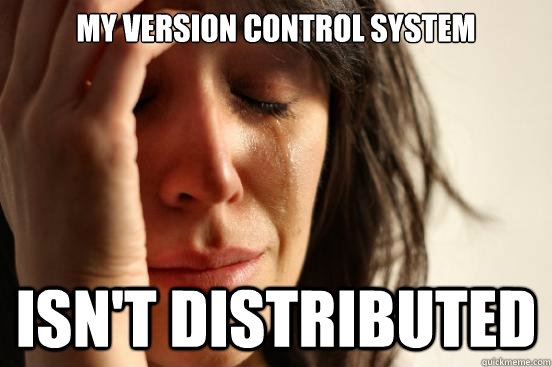
\includegraphics[width=0.8\textwidth]{img/notdistributed.jpg}
    \end{center}
  \end{frame}
}{}

\begin{frame}
  \frametitle{What about a company?}

  Dozens of developers, from several teams:
  \begin{itemize}
    \item working on shared projects
      % 'cause you don't duplicate libs, do you?
    \item modifying the same sources...
    \item ... to serve different purposes
      % features, OS, clients...
  \end{itemize}
  \begin{block}{(Not-so) straightforward solutions}
    \begin{itemize}
      \item versioning hell: duplicate everything
      \item integration hell: designate a \textless \textit{project\_name} \textgreater guru
    \end{itemize}
  \end{block}
\end{frame}

\begin{frame}
  \frametitle{Same code, different delivery flavours}

  Given
  \begin{itemize}
    \item three features \textit{f1, f2, f3}
    \item three clients \textit{A, B, C}
  \end{itemize}
  You may want to provide:
  \begin{itemize}
    \item A: f1, f2, f3
    \item B: f1, f3
    \item C: f2, and a customized f3
  \end{itemize}
  \begin{exampleblock}{Real-world example}
    Web Content Management Systems (CMS): Wordpress, Drupal, MediaWiki...
  \end{exampleblock}
\end{frame}

\begin{frame}
  \frametitle{Getting social}

  We need flexible tools to:
  \begin{itemize}
    \item manage source code
    \item keep track of released versions
    \item allow collaborative work
    \item deliver customized products
  \end{itemize}
  \begin{block}{There comes...}
    \textbf{S}ource \textbf{C}ode \textbf{M}anagement,
    a.k.a. \textbf{V}ersion \textbf{C}ontrol \textbf{S}ystem
  \end{block}
\end{frame}
